\subsection{Comparison between ABC and permABC}
\label{sec:abc_vs_permabc}

As discussed in Section~\ref{sec:comparison}, permABC exhibits a different behavior from standard ABC. In particular, two regimes emerge depending on the value of the threshold \( \varepsilon \): when \( \varepsilon > \varepsilon^* \), permABC yields a different approximation of the posterior compared to ABC; whereas when \( \varepsilon \leq \varepsilon^* \), permABC coincides with standard ABC and thus inherits its convergence guarantees.
% \xian{La question étant quelle approximation est préférable ??}

To better illustrate the differences between the two approaches, we consider a simple toy model with no global parameter, defined as follows:
\[
\mu_k \sim \mathcal{U}(-2, 2), \quad \obsdata_k \sim \mathcal{U}(\mu_k - 1, \mu_k + 1), \quad k = 1, \dots, K,
\]
with \( K = 2 \), and a fixed observation \( y = (-1, 1)^\top \). 

Figure~\ref{fig:unif} highlights the two different regimes. When \( \varepsilon > \varepsilon^* \), permABC is concentrated in a region constrained by the order statistics, leading to a pseudo-posterior different from that of standard ABC. However, when the threshold satisfies \( \varepsilon \leq \varepsilon^* \), both methods recover the same pseudo-posterior. In this example, the critical value is \( \varepsilon^* = \sqrt{1/8}/2 \approx 0.177 \).


Note that, even in its vanilla form, permABC offers a significant gain in simulation efficiency. Since it effectively avoids redundant permutations during rejection, it reduces the required number of simulations by a factor of approximately \( K! \). In this simple example with \( K = 2 \), we achieve the same approximation quality (i.e., same \( \varepsilon < \varepsilon^* \)) using only half the number of simulations compared to standard ABC.

\begin{figure}[htbp]
    \centering
    \includegraphics[scale=.5]{fig/fig3_seed_42.pdf}
    \caption{\old{Comparison between standard ABC (left) and permABC (right) on the toy model of Section \ref{sec:abc_vs_permabc} with \( K = 2 \) and observation \( y = (-1, 1)^\top \). Each dot represents a sampled configuration \( \mu = (\mu_1, \mu_2) \), colored by the acceptance threshold used: purple for \( \varepsilon = \infty \), green for \( \varepsilon > \varepsilon^* \), and yellow for \( \varepsilon = \varepsilon^* \). The black cross denotes the observation \( y \), and the dashed box indicates the true posterior. While both methods recover the same posterior when \( \varepsilon < \varepsilon^* \), permABC avoids simulating permutations that are suboptimal at large \( \varepsilon \), resulting in a more concentrated distribution and improved efficiency. The two panels use the same computational budget.}\new{ABC (left) vs.\ permABC (right) on the uniform toy model with \( K = 2 \). Dots are sampled \( (\mu_1, \mu_2) \) at three tolerance levels: \( \varepsilon = \infty \) (purple), \( \varepsilon > \varepsilon^* \) (green), \( \varepsilon = \varepsilon^* \) (yellow). Both methods agree when \( \varepsilon < \varepsilon^* \); permABC is more concentrated and efficient at equal budget.}}
    \label{fig:unif}
\end{figure}
\subsection{Challenges of High-Dimensional ABC: A Gaussian Toy Model}
\label{sec:gaussian_toy}
We now consider a classical hierarchical model commonly used in the Bayesian literature:
\begin{equation*}
    \label{eqgauss}
    \beta \sim \mathrm{IG}(a,b), \quad \mu_k \sim \mathcal{N}(0, s^2), \quad \obsdata_{k} = (y_{1,k}, \dots, y_{n,k}) \overset{\text{i.i.d.}}{\sim} \mathcal{N}(\mu_k, \beta), \quad k = 1, \dots, K.
\end{equation*}
Throughout this section we set \( a = b = 5 \), \( s = 10 \), \( n = 10 \) observations per component, and \( K = 20 \) unless stated otherwise.

This simple yet representative model provides a convenient testbed to compare the various methods discussed in this paper, and to highlight the limitations of standard ABC approaches in high-dimensional settings. All ABC methods involve a fundamental trade-off between the number of simulations \( N \), the tolerance threshold \( \varepsilon \), and the effective number of accepted samples (or the number of unique particles in sequential schemes). A more efficient method achieves a lower value of \( \varepsilon \) for a given simulation budget \( N \) and fixed final sample size.

To enable fair comparison across methods, we adopt a consistent evaluation criterion: for each experiment, we report the value of \( \varepsilon \) achieved when the algorithm yields exactly 1,000 unique particles. In this setting, the number of simulations required to obtain a single unique accepted sample serves as a proxy for the effective sample size (ESS). This pseudo-ESS provides a normalized measure of sampling efficiency, which we use throughout our benchmarks.

\new{A low tolerance \( \varepsilon \), however, is only a proxy for posterior quality: two methods that target different pseudo-posteriors cannot be compared on \( \varepsilon \) alone. To evaluate the quality of the produced approximation directly, we instead report the sliced Wasserstein-2 distance \citep{bonneel2015sliced,nadjahi2020statistical} between the weighted particle cloud and a reference posterior obtained by long MCMC (PyMC) on the Gaussian toy model of Section~\ref{sec:gaussian_toy}. The sliced Wasserstein metric is well suited to this setting: it metrises weak convergence on \( \mathbb{R}^{d} \), admits linear-time Monte Carlo estimators in the ambient dimension, and has been used as a target discrepancy in ABC by \citet{nadjahi2020approximate}. Reporting \( \mathrm{SW}_2 \) assesses whether the permutation-based gains in tolerance translate into genuinely better posterior approximations.}

Rejection-based algorithms such as vanilla ABC, as well as sequential variants like ABC-SMC and ABC-PMC, are known to scale poorly with the dimension of the parameter space, here indexed by the number of groups \( K \). As \( K \) increases, the acceptance rate drops sharply, resulting in a dramatic rise in computational cost. In contrast, the permutation-based acceptance rule introduced in permABC significantly improves the efficiency of both rejection and sequential samplers in high-dimensional regimes. The symmetry structure across local parameters \( \mu_1, \dots, \mu_K \) allows permABC to reduce redundant simulations and produce sharper approximations of the target pseudo-posterior.

\new{Figure~\ref{fig:vanilla_vs_smc} illustrates this phenomenon in terms of the sliced Wasserstein-2 distance to the reference posterior: permutation-based methods reach substantially lower \( \mathrm{SW}_2 \) values than their non-permuted counterparts at equal simulation budget. In particular, for \( K=20 \) and without outliers, permABC-SMC and permABC-Vanilla plateau roughly \(3\)--\(6\)~times closer to the reference than ABC-SMC or ABC-Vanilla. These gains become increasingly pronounced as \( K \) grows, confirming the advantage of permutation-based strategies in hierarchical or exchangeable models.}

\new{A complementary comparison in terms of wall-clock time — rather than simulation count — yields similar conclusions, and is provided in Appendix~\ref{sec:appendix_comparison}.}

\begin{figure}[htbp]
    \centering
    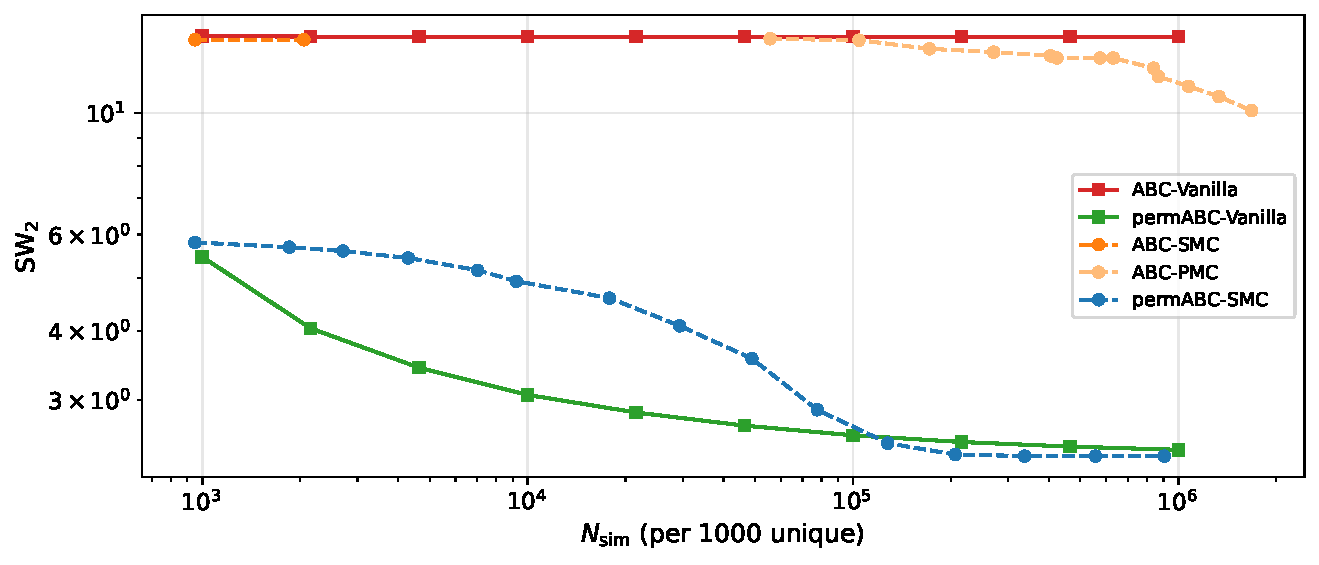
\includegraphics[width=\textwidth]{fig/fig4_sw2_nsim_seed_45.pdf}
    \caption{\new{Sliced Wasserstein-2 distance to the reference posterior vs.\ number of simulations (log--log) for the Gaussian toy model with \( K=20 \), no outliers (\( N_{\mathrm{particles}} = 5{,}000 \)). Permutation-based methods reach substantially lower \( \mathrm{SW}_{2} \) at equal budget. Wall-clock time counterpart in Appendix~\ref{sec:appendix_comparison}.}}
    \label{fig:vanilla_vs_smc}
\end{figure}



\subsection{Failure cases of ABC-Gibbs}
\label{sec:abcgibbs_failure}

ABC-Gibbs methods \citep{clarte2021componentwise,rodrigues2020likelihood} have been designed to handle hierarchical models similar to those we consider. They are however less robust to model dependencies. We illustrate this with a modified hierarchical model designed to highlight the limitations of ABC-Gibbs:
\begin{equation*}
    \label{eqgauss_robin}
    \beta \sim \mathcal{N}(0, 10^2), \quad \mu_k \sim \mathcal{N}(0, 10^2), \quad \obsdata_k = (\obsdata_{1,k}, \dots, \obsdata_{n,k}) \overset{\text{i.i.d.}}{\sim} \mathcal{N}(\mu_k + \beta, 1), \quad k = 1, \dots, K.
\end{equation*}
This model is deliberately over-parameterized: it includes \( K+1 \) parameters for only \( K \) observations. Despite its simplicity, the posterior distribution exhibits a strong ridge structure due to the symmetry between local parameters \( \mu_k \) and the global parameter \( \beta \). This posterior can be reliably approximated using reference MCMC software such as PyMC. 
% \al{closed-form available? — to be computed.}

Figure~\ref{fig:perm_vs_gibbs} shows the two-dimensional marginal posterior over \( (\mu_1, \beta) \) obtained under a fixed simulation budget. While permABC-SMC provides a conservative and coherent approximation of the target posterior—as expected for an ABC method with global proposals—ABC-Gibbs produces a truncated approximation, failing to explore the full posterior support.

\old{This discrepancy is rooted in the very structure of ABC-Gibbs. The algorithm proceeds by sequentially updating each parameter conditionally on the others using ABC rejection steps. In the presence of strong dependencies between parameters, as is the case here, the algorithm exhibits poor mixing: each marginal update is constrained by the current (possibly incorrect) values of the other parameters. As a result, the sampler explores a narrow region of the parameter space, failing to recover the full shape of the posterior.

These results underscore the limitations of coordinate-wise ABC approaches in models with strong local-global coupling. In contrast, permABC-based strategies, which jointly consider the full dataset and parameter configuration at each step, are more robust to such structural challenges.}%
\new{This failure is structural: ABC-Gibbs updates each parameter conditionally on the others, so strong dependencies cause poor mixing. In contrast, permABC jointly considers the full parameter configuration and is robust to such coupling.}




\begin{figure}[htbp]
    \centering
    \includegraphics[scale=.5]{fig/fig5.pdf}
    \caption{\old{Two-dimensional marginal posterior over \( (\mu_1, \beta) \) for the hierarchical model defined in Equation~\eqref{eqgauss_robin}, under a fixed simulation budget. The black ellipses represent level sets of the exact posterior distribution computed via MCMC (PyMC). Blue points correspond to samples produced by permABC-SMC, and red points to those produced by ABC-Gibbs. While permABC-SMC captures the full posterior geometry and respects the strong negative correlation between \( \mu_1 \) and \( \beta \), ABC-Gibbs fails to explore the posterior support. It becomes trapped along a narrow subset of the ridge, leading to a truncated and biased approximation. This illustrates the poor mixing behavior of coordinate-wise ABC samplers in the presence of strong global-local dependencies.}\new{Marginal posterior over \( (\mu_1, \beta) \) for the over-parameterised model~\eqref{eqgauss_robin}. Ellipses: exact MCMC level sets. permABC-SMC (circles) captures the full ridge; ABC-Gibbs (triangles) is trapped in a narrow subset, illustrating poor mixing under strong global--local coupling.}}
    \label{fig:perm_vs_gibbs}
\end{figure}



\subsection{Discussion of the Over-Sampling and Under-Matching Approaches}
\label{sec:osum}

The Over-Sampling and Under-Matching strategies provide two complementary extensions of the permABC framework, each improving robustness and efficiency in different regimes of hierarchical inference under exchangeability.

We evaluate their performance on a Gaussian toy model with \( K = 20 \) compartments, among which 4 have local means \( \mu_k \) lying in the tails of the prior. This setup simulates a realistic scenario involving mild model misspecification or contamination by outliers. \new{Figure~\ref{fig:osum} reports the sliced Wasserstein-2 distance \( \mathrm{SW}_{2} \) between the weighted particle cloud and a reference posterior obtained by long MCMC, as a function of the wall-clock time required to obtain 1{,}000 unique accepted particles. This posterior-quality metric directly measures how close each algorithm gets to the true posterior.}

\new{The Over-Sampling method (permABC-OS) reaches values of \( \mathrm{SW}_{2} \) comparable to standard permABC-SMC at the same runtime, and remains the method of choice in the low-tolerance regime: even though each iteration is more expensive because of larger assignment problems and duplicated particles (see Appendix~\ref{appendix_os}), the additional candidate compartments allow faster progression in the contaminated setting.}

\new{Under-Matching (permABC-UM) is the method that benefits most from the presence of outliers. By relaxing the matching constraint to only \( L<K \) compartments, it allows rapid convergence in \( \mathrm{SW}_{2} \) in the intermediate-tolerance regime while ignoring the worst-matching ones, in line with the behaviour expected from the asymptotic analysis of Section~\ref{sec:permABC_OS}. Empirically, the \( \mathrm{SW}_{2} \) advantage of permABC-UM over permABC-SMC grows almost log-linearly with the number of outliers: on this benchmark, a linear fit on \( \log(\text{ratio}) \) gives a slope of roughly \(-0.12\) to \(-0.16\) per additional outlier for \( K\in\{10,15,20\} \). The same model without contamination does not exhibit such an improvement, confirming that the Under-Matching gain is specifically attributable to outliers. On the other hand, as the algorithm transitions to full matching (\( L_t \to K \)), the acceptance condition tightens and the particle population can degenerate; unlike in the Over-Sampling strategy, this issue cannot be alleviated by duplication, and the method typically fails to reach the lowest \( \mathrm{SW}_{2} \) values.}

These contrasting behaviors suggest that combining the two strategies could yield additional benefits. One possibility is to begin inference with permABC-UM to quickly eliminate poorly fitting regions, then switch to permABC-SMC to refine toward smaller tolerances. More generally, hybrid schemes where \( L_t \) and \( M_t \) are jointly adapted — potentially alternating with changes in \( \varepsilon \) — offer a promising direction for future exploration.

\new{A complementary figure reporting the number of simulations (instead of runtime) is provided in Appendix~\ref{sec:appendix_comparison}.}

\begin{figure}[htbp]
    \centering
    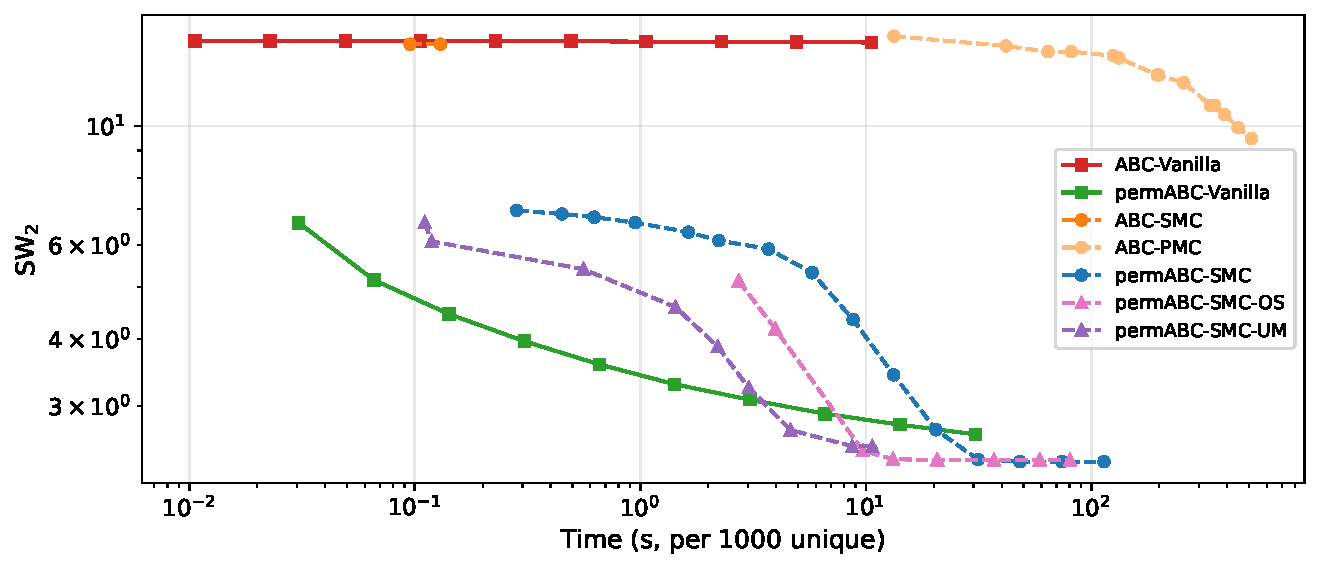
\includegraphics[width=\textwidth]{fig/fig6_sw2_time_seed_45.pdf}
    \caption{\new{\( \mathrm{SW}_{2} \) to reference posterior vs.\ wall-clock time (log--log) for the Gaussian toy model with \( K=20 \) and 4 outliers (\( N_{\mathrm{particles}} = 5{,}000 \)). Under-Matching is most efficient at intermediate tolerances; Over-Sampling remains competitive at low tolerances. Simulation-count counterpart in Appendix~\ref{sec:appendix_comparison}.}}
    \label{fig:osum}
\end{figure}






\subsection{Application to Real Data: The SIR Model}
\label{sec:sir}

In this final section, we illustrate the applicability of our methodology on real-world data by analysing the early spread of COVID-19 in France using publicly available hospitalization records from Santé publique France \citep{DataCovid}. The dataset provides daily hospital admissions at several geographic levels. We focus on mainland France (excluding overseas territories and Corsica), which yields 94 departmental time series.

To describe the epidemic dynamics, we use a classical Susceptible--Infectious--Recovered (SIR) model, defined through the latent system of ordinary differential equations
\begin{equation}
    \label{eqSIR}
    \begin{split}
        \frac{dS}{dt} &= -\delta \frac{SI}{N},\\
        \frac{dI}{dt} &= \delta \frac{SI}{N} - \nu I,\\
        \frac{dR}{dt} &= \nu I,
    \end{split}
\end{equation}
where \(S\), \(I\), and \(R\) denote the numbers of susceptible, infectious, and recovered individuals, respectively, \(N\) is the population size, and \(\delta\) and \(\nu\) are the transmission and recovery rates. The corresponding basic reproduction number is \(R_0 = \delta / \nu\).

\old{Since the available data consist of hospital admissions rather than direct observations of the infectious compartment, the ODE system defines only a latent epidemic trajectory. To obtain simulated datasets, we combine the SIR dynamics with a stochastic observation model. Specifically, the transmission rate at each sub-daily time step is perturbed by a multiplicative log-normal noise:
\[
\delta_k^{(t)} = \delta_k \cdot \exp(\sigma \, \xi_k^{(t)}), \qquad \xi_k^{(t)} \overset{\text{i.i.d.}}{\sim} \mathcal{N}(0,1),
\]
with \(\sigma = 0.05\). This noise captures unmodelled day-to-day variability in transmission---due to reporting delays, local behavioural changes, or stochastic contact patterns---so that the simulated data entering the ABC distance are random even when the underlying SIR dynamics are deterministic. This distinction is important here, as ABC is applied to simulated observations rather than to the deterministic ODE solution itself.}%
\new{Since the data are hospital admissions, the ODE defines a latent trajectory. To introduce stochasticity, the transmission rate is perturbed at each sub-daily step by multiplicative log-normal noise, \(\delta_k^{(t)} = \delta_k \exp(\sigma\,\xi_k^{(t)})\), \(\xi_k^{(t)} \overset{\text{i.i.d.}}{\sim} \mathcal{N}(0,1)\), with \(\sigma = 0.05\). This captures day-to-day variability (reporting delays, behavioural changes, contact patterns), so that the simulated data entering the ABC distance are stochastic.}

\old{To reduce confounding effects due to viral mutations and heterogeneous public-health responses, we restrict attention to the first epidemic wave, from March to July 2020. Over this period, the virus strain and the major national interventions were comparatively homogeneous across departments, making a simplified hierarchical formulation more reasonable.

Initial exploratory analyses (see Appendix~\ref{appendix_sir_validation}) suggest that the basic reproduction number \(R_0\) can be treated as a global parameter shared across departments. For each department \(k=1,\dots,94\), we introduce local parameters
\[
\locparam_k = \bigl(I_k(0), R_k(0), \nu_k\bigr),
\]
while setting \(\delta_k = R_0 \nu_k\). This yields a natural hierarchical structure with exchangeable local parameters and conditional independence across geographic compartments. When defining the distance between observed and simulated datasets (see \eqref{eqdistance}), the weights \(w_k\) may optionally be chosen proportional to the population size of each department in order to account for the different scales of the trajectories.}%
\new{We restrict attention to the first wave (March--July 2020), when the virus strain and national interventions were comparatively homogeneous. Exploratory analyses (Appendix~\ref{appendix_sir_validation}) suggest treating \(R_0\) as a global parameter. Each department \(k=1,\dots,94\) has local parameters \(\locparam_k = (I_k(0), R_k(0), \nu_k)\), with \(\delta_k = R_0\nu_k\), yielding a hierarchical structure with exchangeable locals and conditional independence across compartments.}

\old{This application illustrates the type of high-dimensional hierarchical setting that motivated the development of permABC. With \(K=94\) compartments, three local parameters per department, and one global parameter \(R_0\), the resulting parameter space has dimension
\[
d = 3 \times 94 + 1 = 283.
\]
Such a setting is challenging for standard ABC methods, including sequential variants, because of the curse of dimensionality and the difficulty of efficiently exploring the space of local parameters. By contrast, permABC-SMC can exploit exchangeability across departments and can be combined with the independent-proposal Metropolis-within-Gibbs kernels of Section~\ref{sec:kernels} to perform inference at this scale.}%
\new{With \(K=94\) compartments and three local parameters per department plus \(R_0\), the parameter space has dimension \(d = 3 \times 94 + 1 = 283\). This high-dimensional setting is challenging for standard ABC; permABC-SMC exploits exchangeability and combines with the kernels of Section~\ref{sec:kernels} to perform inference at this scale.}

\old{Figure~\ref{fig_SIR_posterior} illustrates this point by comparing the posterior distributions of \(R_0\) obtained from aggregated national data and from the full collection of departmental trajectories. Using aggregated national data leads to flatter posterior distributions because substantial spatial information is lost. In contrast, the posterior distribution obtained with permABC-SMC from the 94 departmental time series is markedly more concentrated, reflecting the gain from jointly modelling shared global structure and department-specific heterogeneity. The inferred local heterogeneities are shown in the right panel of Figure~\ref{fig_SIR_posterior} and are also mapped geographically in Figure~\ref{fig_SIR_map}.}%
\new{Figure~\ref{fig_SIR_posterior} compares the posterior of \(R_0\) from aggregated national data versus the 94 departmental time series: the departmental posterior is markedly more concentrated, reflecting the gain from jointly modelling spatial heterogeneity. The inferred local recovery rates are mapped in Figure~\ref{fig_SIR_map}.}

\old{Despite these encouraging results, the SIR model remains a highly simplified description of epidemic dynamics and is inevitably misspecified when fitted to real hospitalization time series. In particular, the observation process linking infections to hospital admissions is only coarsely modelled, and many relevant mechanisms---such as reporting effects, delays, behavioural changes, and spatial interactions---are ignored. As a consequence, some posterior estimates of the local recovery rates \(\nu_k\) can take implausibly large values, which should be interpreted as compensating for model misspecification rather than as epidemiologically realistic estimates. This application should therefore be viewed primarily as a proof of scalability and practical relevance for permABC, rather than as a fully realistic epidemiological analysis.}%
\new{The SIR model is inevitably misspecified for real hospitalization data: the observation process is coarsely modelled and many mechanisms (reporting effects, delays, spatial interactions) are ignored. Some estimates of \(\nu_k\) take implausibly large values, compensating for this misspecification. This application should therefore be viewed as a proof of scalability for permABC rather than a fully realistic epidemiological analysis. To confirm that the method itself is sound, Appendix~\ref{appendix_sir_synthetic} presents a synthetic-data experiment with known ground-truth parameters: permABC-SMC recovers the true \(R_0\) and local \(\nu_k\) accurately, together with well-calibrated posterior predictive envelopes, for three values of the noise parameter \(\sigma \in \{0.01, 0.05, 0.10\}\).}

\begin{figure}[htbp]
    \centering
    \begin{subfigure}[t]{0.48\textwidth}
        \centering
        \includegraphics[width=\textwidth]{fig/fig7_posterior_comparison_seed_42.pdf}
        \caption{Posterior for \(R_0\) and \(\nu_k\); departmental (\(K=94\), solid) vs.\ national (\(K=1\), dashed).}
        \label{fig_SIR_posterior}
    \end{subfigure}
    \hfill
    \begin{subfigure}[t]{0.48\textwidth}
        \centering
        
\includegraphics[width=\textwidth]{fig/fig8_map_departmental_seed_42.pdf}
        \caption{Posterior mean \(\nu_k\) by department.}
        \label{fig_SIR_map}
    \end{subfigure}
    \caption{SIR model on French COVID-19 data (\(K=94\) departments, model~\eqref{eqSIR}).}
    \label{fig:sir_combined}
\end{figure}
